\documentclass[First Project.tex]{subfiles}

\begin{document}
\subsection{ Διαγραφή της σελίδας 10 και η επίδραση της στις τάξεις σελίδων  }

Σε αυτή την παράγραφο διαγράφεται η σελίδα $10$ από το υποθετικό μας δίκτυο και αναλύεται η επίδραση αυτής της 
διαγραφής στις τάξεις σελίδων. Αν διαγράψουμε την σελίδα 10 και υπολογίσουμε τις τάξεις σελίδων για το νέο 
δίκτυο παίρνουμε τα αποτελέσματα ( η τάξη της σελίδας 10 εμφανίζεται με $-$ αφού έχει διαγραφεί ) στο 
\textit{Σχήμα 54}.

\begin{figure}[h!]
    \centering
    \captionsetup{justification=centering}
    \begin{center}
        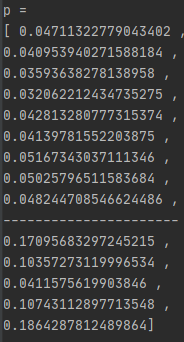
\includegraphics[scale=0.6]{exercise_4_delete_page_10_page_rank.png}    
        \caption{ Τάξη των σελίδων μετά την διαγραφή της σελίδας 10 }
    \end{center}
\end{figure} 

\vspace{10mm}
Όπου παρατηρούμε ότι μειώθηκε η τάξη των σελίδων 9,13 και 14 ενώ των υπολοίπων αυξήθηκαν. Αρχικά, εφόσον η σελίδα
10 δεν υπάρχει πλέον παύει να μεταφέρει την σημαντικότητα της στην σελίδα 13 επομένως η τάξη της σελίδας 13
μειώνεται. Στην συνέχεια αφού μειώνεται η σημαντικότητα της σελίδας 13 και αφού η μόνη σελίδα που δείχνει στην 14 είναι
η 13, μειώνεται και η τάξη της σελίδας 14. Αντίστοιχα, αφού η σελίδα 13 δείχνει και στην 9 μειώνεται και η τάξη της 
σελίδας 9. Από την άλλη μεριά αφού η σελίδα 11 είναι αυτή με τον μεγαλύτερο βαθμό εισόδου που απομένει στο δίκτυο και η
μόνη σελίδα που δείχνει είναι η 15 αυξάνεται ακόμα περισσότερο η τάξη της σελίδας 15, ενώ η σημαντικότητα που είχε και
μετέφερε η σελίδα 10 λόγω του βαθμού εισόδου της, διαμοιράζεται στις σελίδες των οποίων η τάξη ανέβηκε σε σχέση με πριν.
Αυτό μπορούμε να το συμπεράνουμε επίσης αν υπολογίσουμε τη συνολική αύξηση των τάξεων των σελίδων που είναι
$0.2254604468705728$ και τη συνολική μείωση των τάξεων των σελίδων που είναι $0.11912701917096971$. Αν αφαιρέσουμε αυτές
τις δύο τιμές παίρνουμε $0.10633342769960308$, που είναι η τάξη της σελίδας 10 πριν την διαγραφή με αρκετά μεγάλη
ακρίβεια ( περίπου 15 ψηφίων ).

\end{document}